%!TEX program = xelatex
\documentclass[11pt,article,oneside]{memoir}
\usepackage{org-preamble-xelatex}
\DisemulatePackage{setspace}
\usepackage{setspace}
% \input{vc}

\usepackage{longtable}

\usepackage{graphicx}
% We will generate all images so they have a width \maxwidth. This means
% that they will get their normal width if they fit onto the page, but
% are scaled down if they would overflow the margins.
\makeatletter
\def\maxwidth{\ifdim\Gin@nat@width>\linewidth\linewidth
\else\Gin@nat@width\fi}
\makeatother
\let\Oldincludegraphics\includegraphics
\renewcommand{\includegraphics}[1]{\Oldincludegraphics[width=\maxwidth]{#1}}

\title{\bigskip \bigskip How Does the State Speak about Globalisation? A Quantitative Text-Mining
Approach}

%\author{}

\author{\Large Justin Murphy\vspace{0.05in} \newline\normalsize\emph{University of Southampton} \newline\footnotesize \url{j.murphy@soton.ac.uk}\vspace*{0.2in}\newline }

%\author{Justin Murphy (University of Southampton)}

\date{}


\begin{document}  
\setkeys{Gin}{width=1\textwidth} 	
\setromanfont[Mapping=tex-text,Numbers=OldStyle]{Georgia} 
\setsansfont[Mapping=tex-text]{Gill Sans} 
\setmonofont[Mapping=tex-text,Scale=0.8]{Consolas}
\chapterstyle{article-2}

\doublespacing


\maketitle



\begin{abstract}

\noindent Scholars argue that the concept of ``globalisation'' is strategically
deployed by governments to rationalise their actions (Hay and Rosamond
2011). This article is the first large-scale quantitative assessment of
this argument, using text-mining and machine learning techniques to
analyze more than 60,000 government web pages. Specifically, this
article exploits the newly released United Kingdom Government Web
Archive to analyze a random sample of web pages published across the
entire UK government web system between 2000 and 2013.

\end{abstract}


I requested 150,000 web pages, received 67k and about 1k were errors.
Thus, the final sample consists of a corpus of dtm

\pagebreak

\subsubsection{Descriptive Statistics}\label{descriptive-statistics}

\begin{figure}[htbp]
\centering
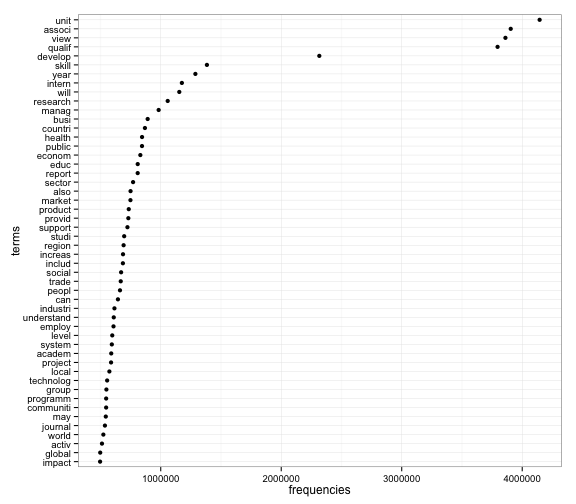
\includegraphics{figure/globalisation_frequency_plot.png}
\caption{Most frequent terms}
\end{figure}

\pagebreak

\paragraph{Correlated terms}\label{correlated-terms}

\begin{longtable}[c]{@{}lr@{}}
\toprule\addlinespace
Terms & Correlation
\\\addlinespace
\midrule\endhead
world & 0.78
\\\addlinespace
countri & 0.66
\\\addlinespace
economi & 0.63
\\\addlinespace
threat & 0.62
\\\addlinespace
increas & 0.61
\\\addlinespace
goal & 0.60
\\\addlinespace
key & 0.60
\\\addlinespace
agricultur & 0.59
\\\addlinespace
also & 0.59
\\\addlinespace
develop & 0.58
\\\addlinespace
particular & 0.57
\\\addlinespace
econom & 0.55
\\\addlinespace
mani & 0.55
\\\addlinespace
privat & 0.55
\\\addlinespace
coher & 0.54
\\\addlinespace
competit & 0.54
\\\addlinespace
primari & 0.53
\\\addlinespace
educ & 0.52
\\\addlinespace
exampl & 0.52
\\\addlinespace
howev & 0.52
\\\addlinespace
integr & 0.52
\\\addlinespace
success & 0.52
\\\addlinespace
capac & 0.50
\\\addlinespace
dfid & 0.50
\\\addlinespace
millennium & 0.50
\\\addlinespace
\bottomrule
\end{longtable}

\paragraph{Cluster Analysis}\label{cluster-analysis}

In this section, I use \emph{k}-means clustering to partition the corpus
of documents into clusters of relatively similar documents. The
\emph{k}-means algorithm, also known as Lloyd's algorithm, is a
non-parametric technique for partitioning \emph{n} observations into the
\emph{k} clusters which minimize within-cluster variance.\footnote{Specifically,
  within-cluster variance refers to the within-cluster sum of Euclidean
  distances from the centroids, or simply within-cluster sum of squared
  error (SSE)}.

K-means cluster analysis requires the analyst to define \emph{k} in
advance. As the number of clusters is typically not known in advance,
the analyst executes the algorithm with several different values for
\emph{k} and compares the within-cluster sum of squared error for each.
The \emph{k} which results in the clusters with the lowest SSE, or is
not significantly improved by additional \emph{k}, is selected as the
optimal \emph{k}. This procedure showed that the 66,400 documents are
optimally partitioned into about 200 clusters.\footnote{See the
  Appendix.}

\pagebreak

\section{Appendix}\label{appendix}

\subsection{Diagnostics}\label{diagnostics}

\begin{figure}[htbp]
\centering
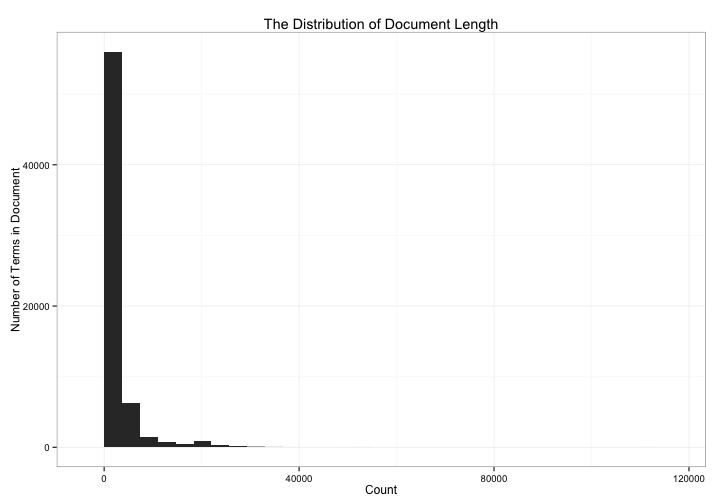
\includegraphics{figure/Document-Lengths.png}
\caption{Document lengths}
\end{figure}

\begin{figure}[htbp]
\centering
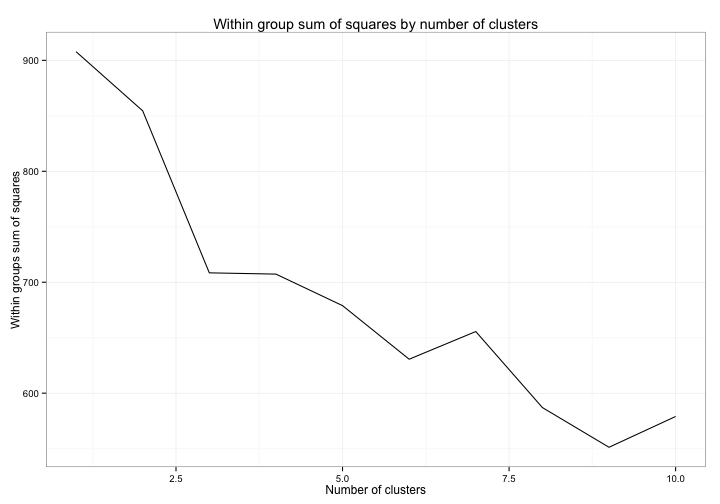
\includegraphics{figure/Cluster-Diagnostics.png}
\caption{plot of chunk Cluster-Diagnostics}
\end{figure}

\pagebreak

\section{References}\label{references}

\setlength{\parindent}{-0.2in} \setlength{\leftskip}{0.2in}
\setlength{\parskip}{8pt} \vspace*{-0.2in} \noindent

Hay, Colin, and Ben Rosamond. 2011. ``Globalization, European
Integration and the Discursive Construction of Economic Imperatives.''
\emph{dx.doi.org.libproxy.temple.edu} 9(2): 147--67.
\url{http://www.tandfonline.com/doi/abs/10.1080/13501760110120192}.


\end{document}